\chapter{Programmbeschreibung zur Flugleistungsberechnung}
\label{chap:Programmbeschreibung}
Im Folgenden wird das Programm, auf dem die Flugleistungsberechnung basiert, beschrieben. Zuerst wird auf die Programmstruktur eingegangen und der Ablauf erörtert (Kap. \ref{sec:aufbau_des_programms}). Im Anschluss erfolgt Aufführung aller Parameter, die das Fluggerät und seine Komponenten definieren, und die Veranschaulichung der grundlegenden mathematischen Zusammenhänge für die Berechnung (Kap. \ref{sec:flugleistungsberechnung}). Zum Schluss wird noch auf die einzuhaltenden Grenzen der Berechnung eingegangen sowie die getroffenen Einschränkungen und Vereinfachungen geschildert (Kap. \ref{sec:vernachlaessigungen_vereinfachungen}).

\section{Aufbau des Programms}
\label{sec:aufbau_des_programms}
Die Leistungsberechnung ist umgekehrt zu einem realen Fluggerät aufgebaut.  Zusammengenommen handelt es sich um den hier beschriebenen Ablauf des Programs zur Flugleistungsberechnung um ein statisches Modell. Dies steht dem realen, dynamischen Verhalten eines Fluggeräts gegenüber. Bei diesem wird über eine Schubhebelstellung die konstante Spannung der Batterie für den Motor moduliert und mit dem Batteriestrom im Motor in eine Leistung umgesetzt, welche den Propeller antreibt. Das Resultat ist der Schub vom Propeller und damit eine Fluggeschwindigkeit.
Der Ablauf des \textsc{Matlab}-Skriptes wird in Abb. \ref{abb:programmstruktur} und der der Leistungsberechnung in Abb. \ref{abb:leistungsberechnung} dargelegt.


\begin{center}
\begin{figure}[H]
\begin{struktogramm}(163,153)
\assign[1]{Fluggerät auswählen und Komponenten definieren(im Startskript)}
\assign[1]{Missions- und Umgebungsparameter festlegen (im Startskript)}
\assign[1]{Diskretisierungen festlegen}
\assign[1]{Aufruf des Hauptskripts: Leistungsberechnung starten}
\assign[1]{Initialisierung der Parameterberechnung}
\while[5]{F\"ur alle Höhenabschnitte}
	\assign[1]{H\"ohe, Dichte, Luftdruck Temperatur berechnen}
	\assign[1]{arithmetische Mittelwert berechnen}
	\assign[1]{Schub- und Leistungskennfeld anpassen}
	\assign[2]{Initialisierung der Leistungsberechnung}
	\while[5]{Für alle Bahnneigungswinkel}
		\assign[2]{\textbf{Flugleistungsberechnung}}
	\whileend
	\ifthenelse[10]{1}{5}{Fluggerät?}{Copter (1)}{Flächenflugzeug (0)}
		\assign[2]{Übergabe der zwischengespeicherten Leistungsparameter}
		\change
		\ifthenelse[10]{5}{1}{Sind die Werte NaN?}{nein}{ja}
			\while[5]{Solange Abbruchkriterium nicht erreicht}		
				\assign[2]{Finde den Index mit der geringsten verbrauchten Energiemenge}
				\ifthenelse[10]{1}{1}{Grenzen überschritten?}{ja}{nein}
				\assign[2]{Verlasse Schleife}
				\change
				\assign[2]{Suche nächst kleinere Energiemenge}
				\ifend
			\whileend
			\assign[2]{Übergabe aller Leistungsparameter mit diesem Index}
			\change
			\assign[2]{Verwerfe alle Ergebnisse}
		\ifend
	\ifend
\whileend
\assign[2]{Ergebnisse der Leistungsparameter in Diagrammen speichern}
\assign[2]{Speichern der Diagramme in .pdf-Datei}
\end{struktogramm}
\caption{Programmablauf}
\label{abb:programmstruktur}
\end{figure}
\end{center}
Das Programm beginnt mit der Festlegung, welches Fluggerät untersucht werden soll (Kap. \ref{subsec:fluggerät}). Anschließend werden alle Parameter des Fluggeräts, der Propeller, der Motoren, der Batterie sowie der Umgebung im Startskript (vgl. Parameter aus Kap. \ref{sec:flugleistungsberechnung}) definiert. Im Hauptskript wird nach der Berechnung sonstiger Parameter und der Initialisierung von Ergebnisvektoren innerhalb einer Schleife die Flughöhe schrittweise erhöht. Für jeden zusätzlichen Höhenschritt werden die Umgebungsbedingungen neu berechnet. Dies umfasst die Dichte, die Temperatur, den Druck und die Schallgeschwindigkeit (Vgl. Kap. \ref{subsec:umgebungsparameter}). Wiederum werden Ergebnisvektoren übergeben. Innerhalb einer weiteren Schleife wird der Bahnneigungswinkel für das Flächenflugzeug variiert. Es folgt die Flugleistungsberechnung (Abb. \ref{abb:flugleistungsberechnung}). 

\begin{center}
\begin{figure}[H]
\begin{struktogramm}(163,140)
\ifthenelse[15]{1}{1}{Fluggerät?}{Copter (1)}{Flächenflugzeug (0)}
			\assign[2]{Berechne Gesamtmasse}
			\assign[2]{Flugzeit für Höhenschritt berechnen}			
			\while[5]{Solange Abbruchkriterium nicht erreicht}
				\assign{Aerodynamik berechnen}
			\whileend
			\assign[2]{Schub berechnen}
			\change
			\assign[2]{Berechne Gesamtmasse}
			\assign[2]{Schub aus Bahnneigungswinkel und Auslegungspunkt berechnen}
			\assign[2]{Flugzeit für Höhenschritt berechnen}
		\ifend
		\assign[2]{Schub auf Propeller verteilen}
		\ifthenelse[10]{1}{4}{Schub zu gro\ss{}?}{ja}{nein}
			\assign[2]{Ergebnis verwerfen (NaN)}
			\change
			\assign[2]{Drehzahl und Drehmoment aus Propellerkennfeld interpolieren}
			\assign[2]{Motorzustand berechnen}
			\assign[2]{Zustand der Motorregler berechnen}
			\assign[2]{Zustand der Batterie neu berechnen}
			\assign[2]{Gesamtwirkungsgrad berechnen}
		\ifend
		\ifthenelse[10]{1}{1}{Werden Grenzen überschritten?}{ja}{nein}
			\assign[2]{Ergebnis verwerfen (NaN)}
			\change
			\assign[2]{Ergebnis beibehalten}
		\ifend
		\ifthenelse[10]{1}{1}{Fluggerät?}{Multicopter (1)}{Flächenflugzeug (0)}
			\assign[2]{break}
			\change
			\assign[2]{Speichern der aufgebrachten Energiemenge}
		\ifend
\end{struktogramm}
\caption{Ablaufstruktur der Flugleistungsberechnung}
\label{abb:flugleistungsberechnung}
\end{figure}
\end{center}

Die Flugleistungsberechnung ist umgekehrt zu einem realen Fluggerät aufgebaut.
Die Berechnung startet mit der Ermittlung des benötigten Schubes für eine vorgegebene Fluggeschwindigkeit innerhalb eines aerodynamischen Modells. Je nachdem welches Fluggerät unterucht wird, unterscheiden sich aerodynamischen Modell für einen Multicopter (Kap. \ref{subsubsec:schub_multicopter}) oder für ein Flächenflugzeug (Kap. \ref{subsubsec:schub_flaechenflzg}). \\
Mit diesem wird der Propellerzustand aus einem Propellerkennfeld, genauer die Drehzahl und das Drehmoment, ermittelt (Kap. \ref{subsec:propellerzustand}). \\
Über die Propellerdrehzahl und -drehmoment errechnet sich der Motorstrom und die Motorspannung, die den Motorzustand bestimmen (Kap. \ref{subsec:motorzustand}). \\
Die Motorzustandsgrößen legen wiederum zum einen die Pulsweitenmodulation und den Wirkungsgrad des Reglers fest (Kap. \ref{subsec:motorreglerzustand}) und zum anderen fließen sie mit diesen Werten in die Berechnung der Batterierestladung ein (Kap. \ref{subsec:batteriezustand}). \\
Im Anschluss an die Flugleistungsberechnung erfolgt die Kontrolle, ob alle errechneten Größen sich innerhalb der Flugenvellope befinden (Kap. \ref{subsec:grenzen}). Ist dies der Fall werden die Ergebnisse beibehalten, ansonsten werden sie verworfen. 
Nach dem Durchlaufen der Iteration über den Bahnneigungswinkel (für einen Multicopter endet diese bereits nach der 1. Iteration, weil der Bahnneigungswinkel mit festgelegten \SI{90}{^\circ} keiner Iteration bedarf) folgt die Auswahl des optimalen Bahnneigungswinkel für das Flächenflugzeug anhand der minimalen aufgebrachten Energie für den jeweiligen Höhenschritt.
Zuletzt werden die Ergebnisse in Diagrammen visualisiert.

%Die Berechnung startet bei der Ermittlung des benötigten Schubes für eine vorgegebene Fluggeschwindigkeit innerhalb eines aerodynamischen Modells. Mit diesem werden aus einem Propellerkennfeld die Drehzahl und das Drehmoment des Propellers bestimmt, welche den Motorzustand definieren. Die Motorzustandsgrößen legen wiederum zum einen die Pulsweitenmodulation und den Wirkungsgrad des Reglers fest und zum anderen fließen sie mit diesen Werten in die Berechnung der Batterierestladung ein.


\section{Flugleistungsberechnung}
\label{sec:flugleistungsberechnung}
Die folgende Flugleistungsberechnung ist äquivalent zum Ablauf innerhalb des Programms (Vgl. Kap. \ref{sec:aufbau_des_programms}) dargelegt. \\
Nach der Festlegung der Fluggeräteart werden die Parameter des Multicopters oder des Flächenflugzeugs zur Charakterisierung dieser bestimmt. Im Anschluss werden die Formeln der Leistungsberechnung dargelegt und letztendlich die technischen Grenzen aufgeführt. 

 
\subsection{Fluggerät}
\label{subsec:fluggerät}
Bei der Auslegung des Fluggeräts werden nicht nur Multicopter betrachtet sondern auch Flächenflugzeuge, sogenannte fixed wing UAVs. Aus diesem Grund sind die Parameter der Propeller, der Motoren, der Batterie und die Umgebungsparameter allgemein für beide Arten der UAVs festgelegt.
Zu Beginn der Mission muss daher das Flugsystem festgelegt werden, da die Berechnung der Aerodynamik entscheidend vom Flugsystem abhängig ist. Die Abfrage erfolgt mit der Variablen \texttt{Abfrage\_Flugsystem}. Diese kann die Werte \texttt{1} für einen Multicopter oder \texttt{0} für ein Flächenflugzeug annehmen.


\subsection{Missionsparameter}
Innerhalb der Flugparameter kann die Nutzlast \texttt{m\_Nutz} des Fluggerätes bestimmt werden. Diese Masse fließt mit der Masse des Fluggerätes, der der Motoren sowie der der Batterie in die Gesamtmasse mit ein. Im Rahmen des Projektes AEROMET UAV ist die Nutzlast auf \SI{250}{g} festgelegt.


\subsection{Umgebungsparameter und Diskretisierung variabler Umgebungsparameter}
\label{subsec:umgebungsparameter}
Für Leistungsuntersuchung wird die Internationale Standardatmosphäre vorausgesetzt. Die Erdbeschleunigung und der Adiabatenexponent werden als konstant über der Höhe angenommen (siehe Tab. \ref{tab:umgebungs_parameter}). Mit Startwerten für die Höhe, die Temperatur, die Dichte und den Luftdruck werden die Abflugbedingungen am Abflugort spezifiziert.  Die Schrittweite der Höhe legt die Genauigkeit der Höhendiskretisierung fest. Die letzten drei Zustandsgrößen stellen wichtige Größen für den Übergang von der Troposphäre in die Stratosphäre dar, die für eine veränderte Berechnung von Temperatur, Dichte und Druck benötigt werden. (Vgl. Gleichung \ref{eq:druck_strato} und \ref{eq:dichte_strato})
\begin{center}
	\captionof{table}{Umgebungsparameter}
	\begin{tabular}{l l l} \hline
		 Parameter & Variablenname & verwendete Größe \\ \hline
		 Erdbeschleunigung \ensuremath{g} & \texttt{g} & \SI{9,81}{m/s^2}  \\
		 Starthöhe \ensuremath{H_0} & \texttt{H\_0} & \si{m} \\
		 Schrittweite der Höhe  \ensuremath{\Delta H} & \texttt{Delta\_H} & \si{m} \\
		 maximale Höhe \ensuremath{H_{max}} & \texttt{H\_max} & \si{m} \\
		 Umgebungstemperatur am Start \ensuremath{T_0} & \texttt{T\_0} & \si{K} \\
		 Luftdruck am Start \ensuremath{p_0} & \texttt{p\_0} & \si{N/m^2} \\
		 Dichte am Start \ensuremath{\rho_0} & \texttt{rho\_0} & \si{kg/m^3} \\
		 Adiabatenexponent \ensuremath{\kappa} & \texttt{kappa} & \SI{1,4}{} \\
		 Gaskonstante der Luft \ensuremath{R} & \texttt{R} & \SI{287}{J/(kg K)} \\
		 Windgeschwindigkeit \ensuremath{u_{Wg}} & \texttt{u\_Wg} & \si{m/s} \\ 
		 Schallgeschwindigkeit \ensuremath{a} & \texttt{a} & \si{m/s} \\
		 Temperatur in \SI{11}{km} Höhe & \texttt{T\_11} & \ensuremath{T_{11} = T_0 - 0.0065\cdot(11000-H_0)} \\
		 Dichte in \SI{11}{km} Höhe & \texttt{rho\_11} & \ensuremath{\rho_{11} = \rho_0\cdot\Big(1 - 0.0065\cdot\frac{11000}{T_0}\Big)^{4.256}} \\
		 Druck in \SI{11}{km} Höhe & \texttt{p\_11} & \ensuremath{p_{11} = p_0\cdot\Big(1 - 0.0065\cdot\frac{11000}{T_0}\Big)^{5.256}} \\ \hline
	\end{tabular}	
	\label{tab:umgebungs_parameter}
\end{center}
\todo[inline]{Entferne alle ensuremath Einheitenbezeichnungen}
Nach der der Internationalen Standardatmosphäre ist der Temperaturkoeffizient bis zur Tropopause in \SI{11}{km} Höhe
\begin{equation}
	\frac{dT}{dH} = -0,0065\frac{K}{m}
\end{equation}
und danach in der unteren Stratosphäre bis zu einer Höhe von \SI{20}{km}
\begin{equation}
	\frac{dT}{dH} = 0 \eqend{.}
\end{equation}
Entsprechend kann der Verlauf der Temperatur, des Druckes und der Dichte von einer Höhe ab \SI{0}{m} bis zur Tropopause mit
\begin{equation}
	T_{0-11} = T_0 - \frac{dT}{dH}\cdot H \eqend{,}
\end{equation}
\begin{equation}
	p_{0-11} = p_0\cdot [1-0,0065\frac{K}{m}\cdot \frac{H}{T_0}]^{5,256} \eqend{,}
	\label{eq:rho_0_11}
\end{equation}
\begin{equation}
	\rho_{0-11} = \rho_0 \cdot [1-\frac{dT}{dH}\cdot \frac{H}{T_0}]^{4,256}
\end{equation}
beschrieben werden. Ab \SI{11}{km} ist der Verlauf von Druck und Dichte durch die Gleichungen
\begin{equation}
	p = p_{11}\cdot e^{\frac{g}{R\cdot T_{11}}\cdot (H-H_{11})} \eqend{,}
	\label{eq:druck_strato}
\end{equation} 
\begin{equation}
	\rho = \rho_{11}\cdot e^{\frac{g}{R\cdot T_{11}}\cdot (H-H_{11})}
	\label{eq:dichte_strato}
\end{equation}
gegeben.
Letztendlich ergibt sich die Schallgeschwindigkeit aus 
\begin{equation}
	a = \sqrt{\kappa\cdot R\cdot T} \eqend{.}
\end{equation}
Um den Einfluss der Flughöhe in der Leistungsberechnung festzuhalten, werden für jedes Höhenintervall die Umgebungsparameter an den oberen und unteren Intervallgrenzen berechnet. Durch Bildung des arithmetischen Mittelwertes ergeben sich daraus durchschnittliche Parameter für den jeweiligen Höhenabschnitt.  

\subsection{Schubberechnung}

\subsubsection{Multicopter}
\label{subsubsec:schub_multicopter}
Die Parameter für den Multicopter sind in Tab. \ref{tab:multicop_parameter} aufgeführt. Die Leermasse fließt mit in die Gesamtmasse mit ein und wird für die Berechnung des Schubs und weiterer Parameter benötigt. Die Beiwerte sind reine Schätzwerte. Für die nachfolgenden Berechnungen ist nur die obere Stirnfläche von Bedeutung, da sich auf diese die Beiwerte als Referenzfläche beziehen. Die Propeller bleiben bei den Stirnflächen unberücksichtigt.
\begin{center}
	\captionof{table}{Parameter des Multicopters}
	\begin{tabular}{l l l} \hline
		 Parameter & Variablenname & verwendete Größe \\ \hline
		 Leermasse des Multicopters \ensuremath{m_{copter}} & \texttt{m\_copter} & \si{kg}\\
		 Obere Stirnfläche \ensuremath{F_{copter,oben}} & \texttt{F\_copter\_oben} & \si{m^2}\\
		 seitliche Stirnfläche \ensuremath{F_{copter,seitlich}} & \texttt{F\_copter\_seitlich} & \si{m^2}\\
		 Oberer Widerstandsbeiwert \ensuremath{c_{W,copter,oben}} & \texttt{c\_W\_copter\_oben} & -\\
		 Seitlicher Widerstandsbeiwert \ensuremath{c_{W,copter,seitlich}} & \texttt{c\_W\_copter\_seitlich} & -\\
		 Maximaler Auftriebsbeiwert \ensuremath{c_{A,copter,max}} & \texttt{c\_A\_copter\_max} & -\\ \hline
	\end{tabular}	
	\label{tab:multicop_parameter}
\end{center}

Der Schub des Multicopters setzt sich zusammen aus dem zu kompensierenden Gewicht und dem Luftwiderstand durch eine Fluggeschwindigkeit. Dazu kommt noch indirekt der ebenfalls zu kompensierende Seitenwind. Innerhalb eines iterativen, aerodynamischen Modells wird der Schub berechnet. Hierbei sind der Auftriebs- und Widerstandsbeiwert Funktionen des modifizierten Anstellewinkels \ensuremath{\alpha_M} (der Schiebewinkel gibt lediglich die Himmelsrichtung der resultierenden Kraft an, welche in diesem Bericht keine Rolle spielt). Die Idee des Aerodynamischen Modells entstammt aus \textcolor{red}{Beyer,Y.2016b}. 
Die Gesamtmasse des Multicopters setzt sich aus der Masse des Rahmens, der Masse der Batterie, der Masse der Motoren und der Nutzlast
\begin{equation}
	m = m_{copter}+m_{Bat}+m_{Mot}\cdot n_{Prop}+m_{Nutz}
	\label{eq:masse_multicopter}
\end{equation}
zusammen.
Die absolute Fluggeschwindigkeit setzt sich zusammen aus Seitenwindgeschwindigkeit und Bahngeschwindigkeit
\begin{equation}
	V_A = \sqrt{(u_{Kg} + u_{Wg})^2+w_{Kg}}
\end{equation}
mit
\begin{equation}
	\begin{pmatrix} u_{Kg} \\ w_{Kg} \end{pmatrix} = \begin{pmatrix}
	\cos\gamma \\ -\sin\gamma	\end{pmatrix} \cdot V_{Kg}.
\end{equation}
Die am Multicopter angreifenden Kräfte werden in Abb.\ref{abb:kraefteggw} dargestellt. 

\begin{figure}[H]
\centering
\begin{small}
	\input{Kraefteggw.pdf_tex}
	\end{small}
	\caption{Kräftegleichgewicht am unbeschleunigten Multicopter unter Berücksichtigung aerodynamischer Kräfte ($k^*$ ist eine beliebige Achse in der $x_f,y_f$-Ebene).}
	\label{abb:kraefteggw}
\end{figure}

Für die spätere Koordinatentransformation wird der Windanstellwinkel
\begin{equation}
	\gamma_a = \arctan \Big(\frac{-w_{Kg}}{u_{Kg}+u_{Wg}}\Big)
\end{equation}
berechnet.
Die iterative Berechnung des modifizierten Anstellwinkels 
\begin{equation}
	\alpha_M = \Theta '-\gamma_a
\end{equation} 
beginnt mit dem Startwert für den Steigungswinkel \ensuremath{\Theta_0'=0}.

Im Anschluss werden die aerodynamischen Beiwerte 
\begin{equation}
	c_W = \frac{c_{W,copter,oben}-c_{W,copter,seitlich}}{2}\cdot \cos(2\cdot \alpha_M)+\frac{c_{W,copter,oben}+c_{W,copter,seitlich}}{2}
\end{equation} und 
\begin{equation}
	c_A = c_{A,max}\cdot \sin(2\cdot \alpha_M)
\end{equation}
berechnet. Auf diese folgt die Berechnung der aerodynamischen Kräfte
\begin{equation}
	W = c_W\cdot \frac{\rho}{2}\cdot F_{copter,oben}\cdot V_A^2, \label{eq:widerstand}
\end{equation}
\begin{equation}
	A = c_A\cdot \frac{\rho}{2}\cdot F_{copter,oben}\cdot V_A^2.
	\label{eq:auftrieb}
\end{equation}
Die aerodynamischen Kräfte werden dann vom aerodynamischen Koordinatensystem in das geodätische Koordinatensystem transformiert:
\begin{equation}
	\begin{pmatrix} X^A \\ Y^A \\Z^A \end{pmatrix}_g = \begin{pmatrix} \cos\gamma_a & 0 & -\sin\gamma_a \\ 0 & 1 & 0 \\ \sin\gamma_a & 0 & \cos\gamma_a \end{pmatrix}^T\cdot \begin{pmatrix} -W \\ 0 \\ -A \end{pmatrix}_a = \begin{pmatrix} -W\cdot\cos\gamma_a-A\cdot\sin\gamma_a \\ 0 \\ W\cdot\sin\gamma_a-A\cdot\cos\gamma_a \end{pmatrix}_g.
\end{equation}
Der Neigungswinkel kann aus dem Kräftegleichgewicht
\begin{equation}
	\Theta_i' = -\arctan\Big(\frac{-X_g^A}{Z_g^A + m\cdot g}\Big), \qquad i =1,2,3,\dots
	\label{eq:neigungswinkel}
\end{equation}
neu berechnet werden und geht als Startwert in den nächsten Iterationsschritt ein. Die Iteration erfolgt solange bis das Abbruchkriterium
\begin{equation}
	\Delta\Theta' = \Theta_i-\Theta_{i-1}\stackrel{!}{<}0,001^{\circ}
\end{equation}
erfüllt wird. 
Ist das Abbruchkriterium erreicht, kann der erforderliche Schub mit dem Satz des Pythagoras aus den Kraftanteilen in \(x_g-\) und \(z_g-\)Richtung
\begin{equation}
	S = \sqrt{{X_g}^2+(Z_g^A+m\cdot g)^2}
	\label{eq:schub_multicopter}
\end{equation}
bestimmt werden.
Für den Fall, dass der errechnete Schub größer als der zur Verfügung stehende Schub ist, wird das Ergebnis verworfen und als \texttt{NaN} (Not a Number) gespeichert.



\subsubsection{Flächenflugzeug}
\label{subsubsec:schub_flaechenflzg}
Mit der Leermasse wird analog zum Multicopter der Schub berechnet (Vgl. Tab. \ref{tab:flugzeug_parameter}). Der zweite Parameter wird zur Bestimmung des aktuellen Flugzustandes benötigt. Dieser ergibt sich aus einem Auslegungszustand mit vorgegebener Gleitzahl \ensuremath{E^\star} und Geschwindigkeit \ensuremath{V^\star} in Bodennähe. Die Bodennähe und die Höhe sind entsprechend durch die Dichte charakterisiert.
\begin{center}
	\captionof{table}{Parameter des Flächenflugzeug}
	\begin{tabular}{l l l} \hline
		 Parameter & Variablenname & verwendete Größe \\ \hline	 
		 Leermasse des Flächenflugzeug \ensuremath{m_{Flugzeug}}& \texttt{m\_Flugzeug} & \si{kg}\\ 
		 Gleitzahl \ensuremath{E} & \texttt{E} & -\\	
		 Auslegungsgleitzahl \ensuremath{E^\star} & \texttt{E\_stern} & - \\
		 Auslegungsgeschwindigkeit \ensuremath{V^\star} & \texttt{V\_stern} & \si{m/s}\\
		 Auslegungshöhe \ensuremath{\rho^\star} & \texttt{rho\_stern} & \SI{1,225}{kg/m^3}\\ \hline
	\end{tabular}	
	\label{tab:flugzeug_parameter}
\end{center}

Zusätzlich wird noch der Bahnneigungswinkel \ensuremath{\gamma} für jeden Höhenschritt diskretisiert. Dabei sollte die Schrittweite so klein wie nötig gewählt werden, um die Genauigkeit zu maximieren und so groß wie möglich, um die Rechendauer akzeptabel gering zu halten. Der Maximalwert entspricht in diesem Fall einem senkrechten Steigflug.
\begin{center}
	\captionof{table}{Diskretisierung des Bahnneigungswinkels}
	\begin{tabular}{l l l} \hline
		 Parameter & Variablenname & verwendete Größe \\ \hline	  
		 Kleinster Bahnneigungswinkel \ensuremath{\gamma_{min}} & \texttt{gamma\_min} & \SI{1}{^\circ}\\	
		 Schrittweite des Bahnneigungsw. \ensuremath{\Delta\gamma} & \texttt{gamma\_Delta} & \SI{1}{^\circ}\\
		 Größter Bahnneigungswinkel \ensuremath{\gamma_{max}} & \texttt{gamma\_max} & \SI{90}{^\circ}\\ \hline
	\end{tabular}	
	\label{tab:flugzeug_parameter}
\end{center}

Der Schub für ein Flächenflugzeug berechnet sich aus der Kompensation des Widerstandes und des Anteils der zu kompensierenden Gewichtskraft. Analog zum Multicopter setzt sich die Gesamtmasse des Flächenflugzeugs aus der Summe aller Komponenten zusammen
\begin{equation}
	m = m_{Flugzeug}+m_{Bat}+m_{Mot}\cdot n_{Prop}+m_{Nutz}.
\end{equation}
Alle Flugzustände eines Flächenflugzeuges können mit den Grundgleichungen der symmetrischen Flugbahn beschrieben werden. Diese Bewegungsgleichungen \cite[S.77]{Bruning.1986} sind
\begin{align}
	m\cdot \dot{V} &= -W + S\cdot\cos(\alpha+\sigma)-m\cdot g\cdot\sin\gamma , \label{eq:widerstandsgleichung} \\ 
	-m\cdot V\cdot\dot{\gamma} &= -A - S\cdot\sin(\alpha+\sigma)+m\cdot g\cdot\cos\gamma , \label{eq:auftriebsgleichung} \\ 
	V\cdot\sin\gamma &= \dot{H}. \label{eq:steiggleichung}
\end{align}	
Für einen stationäre Flug, der im weiteren ausschließlich betrachtet werden soll, gilt \ensuremath{\dot{V} = 0} und \ensuremath{\dot{\gamma} = 0}. Außerdem ist der Winkel (\ensuremath{\alpha + \sigma}) klein, sodass sich mit hinreichender Genauigkeit die Gleichungen \ref{eq:widerstandsgleichung} und \ref{eq:auftriebsgleichung} zu
\begin{equation}
	S = W + \sin\gamma\cdot G, 
	\label{eq:widerstandsgleichung_vereinfacht}
\end{equation}
und
\begin{equation}
	A = m\cdot g\cdot\cos\gamma 
	\label{eq:auftriebsgleichung_vereinfacht}
\end{equation} 
vereinfachen. Der Auslegungspunkt (mit * gekennzeichnet) des Flächenflugzeugs ist ein Horizontalflug (\ensuremath{\gamma^\star = 0}) in Bodennähe bei maximaler Gleitzahl \ensuremath{E^\star} und Geschwindigkeit \ensuremath{V^\star}. Die vereinfachte Auftriebsgleichung \ref{eq:auftriebsgleichung_vereinfacht} vereinfacht sich damit zu
\begin{equation}
	A^\star = m\cdot g .
\end{equation}
Über die Definition der Gleitzahl \cite[S.49]{Bruning.1986}
\begin{equation}
	E = \frac{A}{W}
	\label{eq:gleitzahl}
\end{equation}
berechnet sich der Widerstand mit
\begin{equation}
	W^\star = \frac{A^\star}{E^\star} \eqend{.}
\end{equation}
Unter Annahme eines Fluges im optimalen Operationspunkt, i.e. bei Auslegungsgleitzahl, ist der Nullwiderstand genau die Hälfte des Gesamtwiderstandes \cite[S.82-S.83]{Bruning.1986}
\begin{equation}
	W_0^\star = 0,5\cdot W^\star \eqend{.}
\end{equation}
Es wird vorausgesetzt, dass für jeden Bahnneigungswinkel \ensuremath{\gamma} der Auftriebsbeiwert und folglich der Anstellwinkel konstant bleibt. Dies setzt voraus, dass sich mit ändernder Höhe die Dichte und die Geschwindigkeit ändert, um die obige Voraussetzung zu gewährleisten. Dadurch verringert sich die Geschwindigkeit
\begin{equation}
	V = V^\star\cdot\sqrt{\cos\gamma\cdot\frac{\rho^\star}{\rho}}  \label{eq:geschw_flaechenflugzeug}
\end{equation}
mit einer Vergrößerung der Flughöhe und des Steigwinkels (Herleitung siehe \ref{sec:herleitung_geschw_bez}). Mit dem Staudruck kann der Nullwiderstand 
\begin{equation}
	W_0 = W_0^\star\cdot\frac{V^2\cdot\rho/2}{{V^\star}^2\cdot\rho^\star/2}
\end{equation}
skaliert werden.
Analog zur Berechnung des Widerstandes im Auslegungszustand errechnet sich der Widerstand im aktuellen Betriebspunkt, mit welchem der Flugzustand abgeschätzt werden kann. Dies geschieht nach folgendem Schema
\begin{equation}
Flugzustand\_Flaechenflugzeug = \begin{cases} 
\text{zulässig} & \text{, wenn} \;\;\; W > 2\cdot W_0 \\ 
\text{Grauzone} & \text{, wenn} \;\;\; W_0 < W < 2\cdot W_0 \\ 
\text{vertikaler Steigflug}  & \text{, wenn} \;\;\; W < W_0 
\end{cases}
\end{equation} 
Die Theorie gilt nur für den Bereich kleiner Bahnneigungswinkel. Mit der Variablen \\ \texttt{Flugzustand\_Flaechenflugzeug} wird das Einhalten der Theorie überprüft. Der Fall, dass \ensuremath{W < W_0} beträgt, ist ein Flugzustand, der die Theorie entscheidend verletzt und daher nicht zulässig ist. Ein Flug mit einem Widerstand kleiner als \ensuremath{W_0} ist physikalisch unmöglich.
Letztlich ergibt sich der Schub aus Gleichung \ref{eq:auftriebsgleichung_vereinfacht} und \ref{eq:widerstandsgleichung_vereinfacht}
\begin{equation}
	S = m\cdot g\cdot (\frac{1}{E}\cdot\cos\gamma + \sin\gamma) \label{eq:schub_flaechenflugzeug}
\end{equation}
mit dem Gewicht und Steigwinkel als Variable.
Für \ensuremath{\gamma = 90^\circ} besitzt Gleichung \ref{eq:schub_flaechenflugzeug} eine Definitionslücke. Bei diesem Bahnneigungswinkel müsste der benötigte Schub gerade einmal das Gewicht des Fluggerätes kompensieren. Dabei wird jedoch der Luftwiderstand, der sich aus einer Fluggeschwindigkeit ergibt, vernachlässigt. 
Für den unbeschleunigten, vertikalen Steigflug vereinfachen sich die Widerstandsgleichung \ref{eq:widerstandsgleichung} und die Auftriebsgleichung \ref{eq:auftriebsgleichung} mit den Bedingungen \ensuremath{\dot{V} = 0}, \ensuremath{\dot{\gamma} = 0}, \ensuremath{\gamma = 90^\circ} und \ensuremath{(\alpha + \sigma) \approx 0} zu 
\begin{equation}
	S = W + G \eqend{,} 
\end{equation}
\begin{equation}
	A = 0 \eqend{.}
\end{equation}
Da der Auftrieb Null ist, erfolgt der unbeschleunigte, vertikale Steigflug mit dem Nullwiderstand
\begin{equation}
	W = W_0 \eqend{.}
	\label{eq:widerstand_vertikalflug}
\end{equation}
Den Bahnneigungswinkel \ensuremath{\gamma} gilt es in jedem Höhenschritt zu optimieren, in dem die Theorie nicht verletzt wird (\texttt{Flugzustand\_Flaechenflzg} = vertikaler Steigflug). Im Falle des vertikalen Steigflugs ist eine Variation der Steiggeschwindigkeit von Interesse. Deshalb werden beide in Abhängigkeit des Flugzustandes für einen Höhenschritt variiert. Maximum der Geschwindigkeitsuntersuchung für einen vertikalen Steigflug ist die Auslegungsgeschwindigkeit \ensuremath{V^\star}. Das Auswahlkriterium ist die für den Höhengewinn benötigte Energiemenge, die sich aus dem Produkt der entnommenen Batteriekapazität und der Batteriespannung zusammensetzt
\begin{equation}
	\Delta = \Delta C_{Bat}\cdot U_{Bat}.
\end{equation}
Die minimal aufgebrachte Energie legt am Ende den besten Steigwinkel fest.
Der Windeinfluss kann in diesem Modell vorerst vernachlässigt werden. Laterale Winde haben keinen Einfluss auf die Steigzeit oder die zum Steigen benötigte Energiemenge. Jedoch verändern die Winde die zurückglegte Strecke über Grund für eine gewisse Höhendistanz \cite[S.241-242]{Scheiderer.2008}. Diese ist für eine Betrachtung Flächenflugzeuges vorerst ohne Belang. 


\subsection{Propellerzustand}
\label{subsec:propellerzustand}

Der Propellername wird in der Form 'Durchmesser x Steigung' angegeben (siehe Tab. \ref{tab:prop_parameter}). Der Name ist wichtig, um das Propellerkennfeld aus der Propellerdatenbank von APC \cite{apc} zu entnehmen. Die Anzahl der Propeller beeinflusst entscheidend die Geometrie des Fluggerätes. Weiterhin wird damit der benötigte Schub auf die Anzahl der Propeller aufgeteilt.
\begin{center}
	\captionof{table}{Propellerparameter für Schub, aerodynamische und technische Grenzen}
	\begin{tabular}{l l l} \hline
		 Parameter & Variablenname & Einheit \\ \hline
		 Propellername & \texttt{prop\_name} & - \\
		 Anzahl der Propeller \ensuremath{n_{Prop}} & \texttt{n\_Prop} & - \\ 
		 Propellerradius & \texttt{r} & \ensuremath{r = D\cdot 0,0254/2} \\
		 Fläche eines Propellers & F & \ensuremath{F = \pi\cdot r^2} \\\hline
	\end{tabular}	
	\label{tab:prop_parameter}
\end{center}

In der Propellerdatenbank vom Propellerhersteller APC sind zu jedem Propeller dieser Marke die Kennfelder angegeben. Diese Kennfelder enthalten für eine Drehzahl die Geschwindigkeiten, Fortschrittsgrade, Schub- und Leistungsbeiwerte, Schub und Leistung sowie weitere Kenngrößen, die innerhalb des "`NASA Transonic Airfoil Analysis Computer Program"\; numerisch berechnet wurden \cite{apc.theory}. Ein beispielhaftes Kennfeld ist in \ref{sec:propellerkennfeld} dargelegt. Die Art der Aufführung lässt allerdings keine Interpolation der Drehzahl bzw. des Drehmomentes in Abhängigkeit des Schubes und der absoluten Fluggeschwindigkeit zu. Aus diesem Grund muss das Kennfeld auf äquidistante Geschwindigkeitsabstände transformiert werden. Dazu wird ein Geschwindigkeitsvektor mit Abständen von \SI{1}{m/s} gebildet. Die Funktion \texttt{Propeller\_map} (entommen aus Beyer, Y. (2016)) interpoliert danach das Schub- und Leistungskennfeld neu über der Geschwindigkeit und Drehzahl. Mit dem zuvor berechneten Schub und der absoluten Fluggeschwindikeit kann schließlich mit der Funktion \texttt{Propeller} die Drehzahl und das Drehmoment mittels linearer Interpolation ermittelt werden.
Die Kennfelder wurden in Versuchen ermittelt, die keine ändernde Dichte berücksichtigen. Um den Einfluss der sich verringernden Dicht mit zunehmender Flughöhe trotzdem zu beachten, müssen die Kennfelder angepasst werden. Gemäß der Strahltheorie setzt sich der Schub aus dem Massenstrom und der Geschwindigkeit im voll ausgebildeten Abstromzylinder 
\begin{equation}
	S =  \dot{m}\cdot w_{i,f\infty} = \rho\cdot A_{Propeller}\cdot w_{i,f}\cdot w_{i,f\infty}
	\label{eq:propellerschub}
\end{equation}
zusammen. Unter der Annahme vernachlässigbar kleiner Differenzen von  induzierten Geschwindigkeiten \ensuremath{w_{i,f}} und Geschwindigkeiten im voll ausgebildeten Abstrom \ensuremath{w_{i,f\infty}} kann das Schubkennfeld des Propellers an den Höheneinfluss 
\begin{equation}
	\frac{S_1}{S_2} = \frac{\rho_1}{\rho_2}
\end{equation}
angepasst werden. Diese Beziehung gilt analog für die Leistung und das Drehmoment. 
Bei den hohen Drehzahlen des Propellers können Machzahleffekte auftreten. Um dies zu kontrollieren wird zusätzlich noch die Blattspitzengeschwindigkeit berücksichtigt
\begin{equation}
	Ma_{tip} = \frac{\Omega\cdot r}{a} \eqend{.}
\end{equation}

Der Propellerwirkungsgrad \ensuremath{\eta_{Prop}} 
\begin{equation}
	\eta_{Prop} = \frac{P_{Strahl}}{P_{Welle}}
	\label{eq:eta_prop}
\end{equation}
setzt die erzeugte Strahlleistung 
\begin{equation}
	P_{Strahl} = S\cdot (w_{i,f}+ w_{Af})
	\label{eq:strahlleistung}
\end{equation}
in Bezug zur Wellenleistung
\begin{equation}
	P_{Welle} = \Omega \cdot M \eqend{.}
\end{equation} 
Zur Berechnung der induzierten Geschwindigkeit im Steigflug wird das Newton-Raphson-Verfahren herangezogen. Mit diesem lässt sich innerhalb weniger Iterationsschritte die induzierte Geschwindigkeit im Steigflug ermitteln \cite[S.153]{Wall.2015}. Im Gegensatz zu van der Wall wird an dieser Stelle mit den senkrecht durch die Propellerebene gehenden Geschwindigkeiten \ensuremath{w_{ges,f} = w_{i,f} + w_{Af}} gerechnet:
\begin{equation}
	(w_{i,f} + w_{Af})_{n+1} = w_{i,f,n} - \frac{w_{i,f,n}}{w_{i,f,n-1}}, \;\;\; n = 0,1,2,\dots
\end{equation}
mit 
\begin{equation}
	f = w_{i,f,n} - w_{Af} - \frac{w_{i0,f}}{\sqrt{u_{A,f}+w_{i,f,n}}} \;\;\; \text{und} \;\;\; f'=1 + w_{i,f,n}\cdot\frac{w_{i0,f}}{\sqrt[3]{u_{Af}+w_{i,f,n}}} \eqend{.}
\end{equation}
Dabei ist 
\begin{equation}
	u_{Af} = V_{A}\cdot\cos\alpha_{M}
\end{equation}
die laterale Komponente entlang der Propellerebene und 
\begin{equation}
	w_{Af} = - V_{A}\cdot\sin\alpha_{M}
\end{equation}
und die vertikale Komponente der Propelleranströmung durch die Rotorebene. Den Startwert der Iteration stellt die induzierte geschwindigkeit im Schwebeflug \ensuremath{(w_{i,f}+w_{Af})_{0} = w_{i0,f}} dar. Hierbei ist darauf hinzuweisen, dass für \ensuremath{w_{Af}} die Vorzeichenkonvention nach \cite{Wall.2015} gewählt wurde, was einem umgedrehten Vorzeichen zur LN 9300 entspricht. 


\subsection{Motorzustand}
\label{subsec:motorzustand}
Manche Motorbezeichnungen erfolgen nach der Form "`AXI 2814/20 GOLD LINE"\; (Die Werte stehen für Statordurchmesser: \SI{28}{mm}, Statordicke: \SI{14}{mm}, Windungszahl: 20). 
Die ersten drei Motorparameter in Tab. \ref{tab:mot_parameter} sind notwendig, um den Motorzustand zu berechnen. Der vorletzte Parameter dient als technische Grenze, die für ein gut ausgelegtes System nicht überschritten wird. Die Motormasse fließt in Kombination mit der Anzahl der Propeller in die Gesamtmasse des Fluggerätes mit ein. Die vorrangige technische Leistungsgrenze ist ist die maximale Motorleistung, die durch den maximalen Motorstrom \ensuremath{I_{max}} repräsentiert wird \cite{axi}. 

\begin{center}
	\captionof{table}{Motorparameter für technische Grenzen}
	\begin{tabular}{l l l} \hline
		 Parameter & Variablenname & Einheit \\ \hline
		 Innenwiderstand \ensuremath{R_i} & \texttt{R\_i} & \SI{}{\ohm} \\
		 Geschwindigkeitskonstante \ensuremath{K_V} & \texttt{K\_V} & \ensuremath{\frac{RPM}{V}} bzw. \SI{}{U/Vs} \\
		 Leerlaufstrom \ensuremath{I_0} & \texttt{I\_O} & \SI{}{A}  \\
		 maximaler Dauerstrom \ensuremath{I_{max}} & \texttt{I\_max} & \SI{}{A} \\
		 Motormasse \ensuremath{m_{Mot}} & \texttt{m\_Mot} & \SI{}{kg} \\ \hline
	\end{tabular}	
	\label{tab:mot_parameter}
\end{center}

Mit dem Drehmoment und der Drehzahl des Propellers berechnet sich der Motorzustand, genauer der Motorstrom und die Motorspannung. Dies erfolgt nach einem einfachen Motormodell \cite{Drela.2007} (siehe dazu auch \ref{sec:motormodell}.
Der Motorstrom berechnet sich aus 
\begin{equation}
	I_{Mot} = Q\cdot K_v + I_0. \label{eq:motorstrom}
\end{equation}
Mit dem Strom ergibt sich die Spannung zu
\begin{equation}
	U_{Mot} = \frac{\Omega}{K_v} + R_i\cdot I_{Mot} \eqend{.} \label{eq:motorspannung}
\end{equation}
Der Wirkungsgrad ist für den Motor das Verhältnis aus der Wellenleistung am Propeller zur elektrischen Leistung, dem Produkt aus Motorspannung \ensuremath{U_{Mot}} und Motorstrom \ensuremath{I_{Mot}}
\begin{equation}
	\eta_{Mot} = \frac{M\cdot\Omega}{U_{Mot}\cdot I_{Mot}} \eqend{.}
	\label{eq:eta_mot}
\end{equation}


\subsection{Zustand der Motorregler}
\label{subsec:motorreglerzustand}
Das Modell der Wirkungsgradsberechnung von bürstenlosen Gleichstrom-Motorreglern (Electronic Speed Control (ESC)) stammt aus \textcolor{red}{Lubrano 2016} und wird auch in \textcolor{red}{Beyer 2016b} verwendet. Hiernach berechnet sich der Wirkungsgrad 
\begin{equation}
\eta_{ESC} = \begin{cases} 
0,7\cdot \text{PWM} + 0,50 & \text{, wenn} \;\;\; 0 < \text{PWM} \leq 0,5 \\ 
0,2\cdot \text{PWM} + 0,75 & \text{, wenn} \;\;\; 0,5 < \text{PWM} \leq 1 \\ 
\text{undefiniert} & \text{, sonst} 
\end{cases}
\label{eq:eta_pwm}
\end{equation} 
mit der Pulsweitenmodulation (PWM) 
\begin{equation}
	PWM = \frac{U_{mot}}{U_{Bat}} \eqend{,}
	\label{eq:pwm}
\end{equation}
die sich aus dem Spannungsverhältnis des ESCs zusammensetzt.


\subsection{Batteriezustand}
\label{subsec:batteriezustand}

Die in Tab. \ref{tab:bat_parameter} aufgeführten Parameter der Batterie bestimmen zum einen die verfügbare Kapazität und zum anderen die Batterieentladung. Bei der Energiedichte handelt es sich um repräsentative Werte für den verwendeten Akkutyp, z.B. Li-Ion oder Li-Po. Dieser Wert errechnet sich aus den verwendeten Batteriezellen \cite{batteriezelle}, die in Kap. \ref{chap:nachbildung_des_quadrocopter} verwendet werden
\begin{equation}
	\omega = \frac{\SI{3.12}{Ah}\cdot \SI{3600}{s/h}\cdot \SI{3,7}{V}}{\SI{0.0466}{kg}} \eqend{.}
\end{equation}
Die minimale Zellenspannung ist ein Erfahrungswert, der am \textit{Institut für Flugführung} verwendet wird. Die maximale C-Rate dient als weitere technische Begrenzung, die wiederum für ein gut ausgelegtes System nicht erreicht wird. Der letzte Parameter stellt eine wichtige Begrenzung dar.
Häufig werden Batterien z.B. in der Form 4s3p angegeben. Diese Angabe beschreibt die Bauform der Batterie. Dabei enthält die Batterie insgesamt 12 (\ensuremath{4\cdot 3}) Zellen, wobei 4 seriell (s) und 3 Zellen parallel (p) angeschlossen sind. Die seriell angeschlossenen Batteriezellen definieren die nominelle Batteriespannung, in diesem Fall \ensuremath{4\cdot \SI{3,7}{V}} also \SI{14,8}{V}. Dahingegen bestimmen die parallel geschalteten Zellen die Kapazität (z.B. \ensuremath{3\cdot \SI{3}{Ah} = \SI{9}{Ah}}).

\begin{center}
	\captionof{table}{Batterieparameter zur Berechnung der verbleibenden Restladung sowie der technischen Grenzen}
	\begin{tabular}{l l l} \hline
		 Parameter & Variablenname & Einheit \\ \hline
		 Energiedichte \ensuremath{\frac{E_{Bat}}{m_{Bat}}}& \texttt{E\_Dichte} & \SI{890540}{J/kg} \\
		 Anzahl der Batteriezellen \ensuremath{N_{Bat,cell}} & \texttt{N\_bat\_cell} & - \\
		 nominale Spannung pro Batteriezelle \ensuremath{U_{Bat,cell}} & \texttt{U\_bat\_cell} & \SI{3,7}{V} \\
		 minimale Spannung pro Batteriezelle \ensuremath{U_{Bat,cell,min}} & \texttt{U\_bat\_cell\_min} & \SI{3,1}{V} \\
%		 Peukert-Konstante \ensuremath{P}& \texttt{P\_bat\_Peukert} & \ensuremath{1,05} \\
		 Maximale C-Rate \ensuremath{\dot{C}_{Rate,max}} & \texttt{C\_Rate\_max} & \SI{}{1/h} \\
		 Batteriemasse \ensuremath{m_{Bat}} & \texttt{m\_bat} & \SI{}{kg} \\ 
		 Nominale Batteriespannung & \texttt{U\_Bat\_nom} & \ensuremath{U_{Bat,nom} = N_{Bat,cell}\cdot U_{Bat,cell}} \\
		 Minimale Batteriespannung & \texttt{U\_Bat\_min} & \ensuremath{U_{Bat,min} = N_{Bat,cell}\cdot U_{Bat,cell,min}} \\ 
		 normierte Batteriekapazität \ensuremath{C_{Bat,normiert}} & \texttt{C\_nomiert} & - \\ \hline
	\end{tabular}	
	\label{tab:bat_parameter}
\end{center}
%Um den Energieverlust der Batterie zu berechnen, wird die Peukert-Konstante herangezogen. Diese beträgt für Li-Po-Akkus ca. $1,01 \leq P \leq 1,05$ und für Li-Ion-Akkus ca. 1,05 (\textcolor{red}{Traub} Blub). Außerdem ist die Peukert-Konstante für Li-Po-Batterien von der Temperatur abhängig. Niedrigere Temperaturen als die Umgebungstemperatur können die angegebene Nennkapazität reduzieren und die Batterieverluste progressiv steigen lassen.


\subsubsection{Normzelle}
Bei Batterien, dies schließt Li-Po und Li-Ion Batterien mit ein, ist eine Abhängigkeit der Batteriespannung von der Entladerate und von der Zeit zu verzeichnen. Eine Möglichkeit dies zu berücksichtigen ist die Verwendung der Peukert-Konstante, die die nutzbare oder nominelle Batteriekapazität reduziert. Die Peukert-Konstante ist abhängig vom Batterietypen und vom gewählten Modell. Für Li-Ion und Li-Po-Batterien liegt diese für gewöhnlich zwischen $1,01 \leq P \leq 1,05$ für Li-Po und bei ca. 1,05 für Li-Ion \cite{Traub.2016}. Hierbei ist eine Kenntnis über die Entladekurve keine Voraussetzung, weswegen die Verwendung der Peukert-Konstante ein sehr einfaches Modell darstellt. 
Daher wird an dieser Stelle ein Modell verwendet, das die Entladkurve (Vgl. Abb. \ref{abb:discharge_curve}) der Batterie berücksichtigt \cite{Tremblay.2009} und somit auch die oben genannten Batteriespannungsabhängigkeiten.  
\begin{figure}[H]
	\centering
	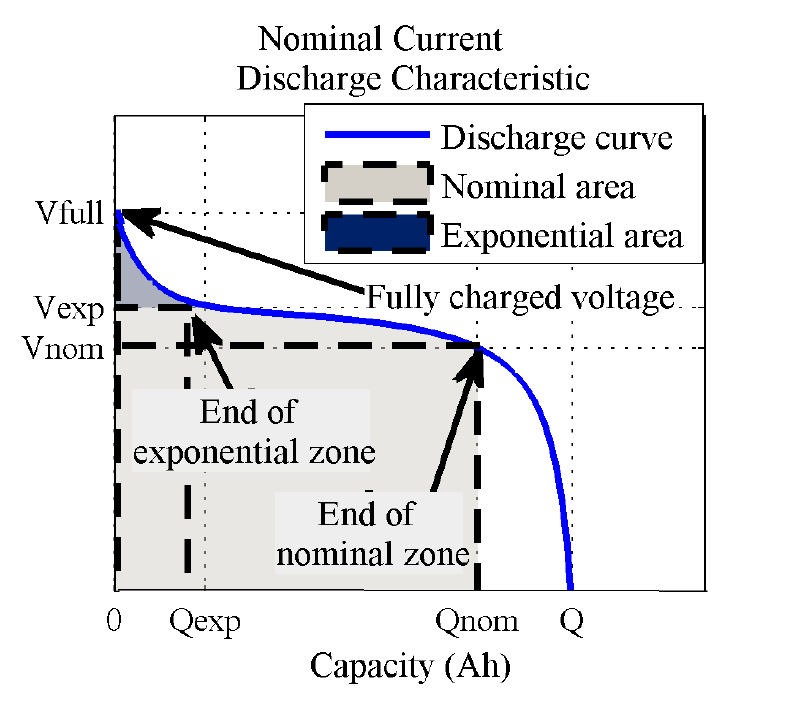
\includegraphics[scale=0.5]{images/Discharge.PNG}
	\caption{Typische Entladekurve für eine Li-Po-Batterie \cite{Tremblay.2009}}
	\label{abb:discharge_curve}
\end{figure}

Die Entladekurve für Li-Po-Batterien kann mit folgender Gleichung beschrieben werden
\begin{equation}
	U_{bat} = E_0-K\cdot\frac{C_{Bat}}{C_{Bat}-\int_{}^{} I_{Bat} dt}\cdot\int_{}^{} I_{Bat} dt - R_{i}\cdot I_{Bat}+A\cdot e^{-3\cdot\int_{}^{} I_{Bat} dt}-K\cdot\frac{C_{Bat}}{C_{Bat}-\int_{}^{} I_{Bat} dt}\cdot I_{Bat}^* \label{eq:batteriespannung}
\end{equation}
Dabei ist \ensuremath{E_0} die konstante Batteriespannung, \ensuremath{K} die Polarisationskonstante, \ensuremath{C_{Bat}} die Batteriekapazität, \ensuremath{\int_{}^{} I_{Bat} dt} die tatsächliche Batterieladung, \ensuremath{A} die Amplitude der Exponentiellen Methode, \ensuremath{B} die inverse Zeitkonstante der exponentiellen Zone, \ensuremath{R_{i}} der Innenwiderstand, \ensuremath{I_{Bat}} der Batteriestrom und \ensuremath{I_{Bat}^\star} der gefilterte Strom (in diesem Fall \(= 0\)). \\
Li-Po Batterien weisen ein der Li-Ion Batterie ähnliches Verhalten auf, weshalb beide nach \ref{eq:batteriespannung} berechnet werden können.\\
Die unbekannten Parameter \ensuremath{E_0}, \ensuremath{A} und \ensuremath{K} können mithilfe von drei Punkten \ensuremath{V_{full}}, \ensuremath{V_{exp}}, \ensuremath{V_{nom}} und die Kapazität \ensuremath{Q}, \ensuremath{Q_{exp}} und \ensuremath{Q_{nom}} (vgl. Abb. \ref{abb:discharge_curve}) bestimmt werden. Diese drei Punkte entstammen von den experimentell gemessenen Entladekurven \cite{elektromodellflug}.
Die Bestimmung der unbekannten Parameter geschieht mit dem gegebenen Innenwiderstand \ensuremath{R_{Bat}} nach folgendem Schema:
\begin{equation}
	\begin{pmatrix} E_0 \\ A \\ K \end{pmatrix} = \textbf{A}^{-1}\cdot \begin{pmatrix}
	V_{full}+R\cdot I_{Bat} \\ V_{exp}+R\cdot I_{Bat} \\ V_{nom}+R\cdot I_{Bat} \end{pmatrix}\; ,
\end{equation}
mit der Beziehung
\begin{equation}
	\textbf{A} = \begin{pmatrix}
	1 & 1 & 0 \\ 1 & e^{-3} & -\frac{Q\cdot (Q_{exp}+I_{Bat})}{Q-Q_{exp}} \\ 1 & e^{-3\cdot\frac{Q_{nom}}{Q_{exp}}} & -\frac{Q\cdot (Q_{exp}+I_{Bat})}{Q-Q_{exp}}
	\end{pmatrix}\; .
\end{equation}
Die experimentellen Entladekurven stammen aus der Datenbank von \cite{elektromodellflug}. In dieser Datenbank sind viele verschiedene Batterien enthalten, die sich in Bezug auf den Hersteller, der Anzahl der Batteriezellen, der Kapazität, der maximalen Entladerate, dem Gewicht, dem Innenwiderstand etc. unterscheiden. Dies erschwert es allgemeine Aussagen über die Batterie unabhängig von der Batteriequalität des Herstellers und der ihrer Größe zu treffen. \\
Für die nachfolgende Untersuchungen ist es daher interessant, eine normierte Batteriezelle zu erstellen, die unabhängig von den oben genannten Unterschieden verwendbar ist. Mit dieser Zelle kann jede beliebige Batteriegröße modelliert werden. \\
Die Batteriekapazität jeder Batterie aus der Datenbank werden mit \SI{1}{Ah} normiert
\begin{equation}
	C_{Bat,nomiert} = \frac{C_{Bat}}{\SI{1}{Ah}}\; .
\end{equation} 
Die drei Punkte für die Spannung \ensuremath{V_{full}}, \ensuremath{V_{exp}} und \ensuremath{V_{nom}} in der Datenbank sind bereits auf eine Batteriezelle bezogen und entziehen sich somit einer Normierung. 
Für jede Batterie werden die drei Spannungspunkte \ensuremath{Q}, \ensuremath{Q_{exp}} und \ensuremath{Q_{nom}} auf eine Batteriezelle bezogen und anschließend mit der normierten Batteriekapazität \ensuremath{C_{Bat,nom}} normiert. 
Über alle Batterieparameter der in der Datenbank enthaltenen Batterien wird der arithmetische Mittelwert gebildet. 
Die gilt nicht für den Entladestrom \ensuremath{i} und den Innenwiderstand \ensuremath{R_{i}}. Alle Werte der drei Punkte (\ensuremath{V_{full}}, \ensuremath{V_{exp}}, \ensuremath{V_{nom}} und die Kapazität \ensuremath{Q}, \ensuremath{Q_{exp}} und \ensuremath{Q_{nom}}) sind bei einer Entladerate \ensuremath{\dot{C}} von \SI{10}{1/h} gemessen worden. Daher entspricht der Entladestrom nach der Normierung genau 1/100 der ursprünglichen Kapazität.
Weil diese für jede Batterie gilt, muss auch dieser nicht gemittelt werden. 
Die Annahme eines konstanten, gemittelten Innenwiderstandes für alle Batteriezellen führt zu signifikanten Diskrepanzen zwischen der Norm- und Originalzelle. 
Wird der Innenwiderstand in Abhängigkeit der Kapazität und der maximalen C-Rate gesetzt, so kann eine hyperbolische Abhängigkeit von beiden Größen festgestellt werden. 
Mithilfe der \textsc{Matlab} Curve Fitting Toolbox kann der Abhängigkeit en Funktionstyp der Form
\begin{equation}
	f(C_{Bat},\dot{C}) = \frac{k}{C_{Bat}\cdot(a\cdot C_{Bat}+b\cdot \dot{C})^c}
\end{equation}
zugrunde gelegt werden. 
Die unbekannten Konstanten ergeben sich dabei zu k = 0,1077, a = 0,1555, b = 0,9825 und c = 0,5485. Zur Steigerung der Genauigkeit werden einige Batteriezellen aus der Berechnung der Erstellung dieses Modells herausgenommen, da diese erhebliche Abweichungen von der Standardabweichung aufzeigen. Dies bezieht sich vor allem auf einzellige Batterien mit einer vergleichsweise geringen Kapazität und sehr hohem Innenwiderstand. Deshalb sei hier angemerkt, dass sich dadurch die Genauigkeit vor allem im Bereich kleiner C-Raten und Kapazitäten verringert.
Der Vergleich der Normzelle zur Originalzelle (Siehe \ref{sec:norm_vs_orig}) zeigt auf, dass die Spannung der Normelle im Durchschnitt etwa \SI{14}{\%} geringer ist als die der Originalzelle. Dies ist bei der Auswertung zu berücksichtigen.


\subsubsection{Batteriezustand}
Die wesentlichen Zustandsgrößen der Batterie stellen der Entladestrom der Batterie \ensuremath{I_{Bat}} und die Batteriespannung \ensuremath{U_{Bat}}

Der Batteriestrom setzt sich zusammen aus den Motorströmen und zusätzlich aus dem Wirkungsgrad der PWM
\begin{equation}
	I_{Bat} = I_{Mot}\cdot \frac{PWM}{\eta_{PWM}}\cdot n_{Prop}.  \label{eq:batteriestrom}
\end{equation}
Die C-Rate \ensuremath{\dot{C}} [1/h] berechnet sich nach 
\begin{equation}
	\dot{C} = \frac{I_{Bat}[A]}{C_{Bat}[As]}\cdot 3600[s/h]
	\label{eq:c_rate}
\end{equation}
Die Ermittlung der zweiten Zustandsgröße erfolgt nach Gleichung \ref{eq:batteriespannung} für die genormte Batteriezelle. Hierfür ist der Batteriestrom vorher zu normieren
\begin{equation}
	I_{Bat,normiert} = \frac{I_{Bat}}{C_{Bat,normiert}} \eqend{.}
\end{equation}
Die Gesamtbatteriespannung ergibt sich am Ende aus der Summe aller Zellspannungen
\begin{equation}
	U_{Bat} = N_{Bat,cell}\cdot U_{Bat} \eqend{.}
\end{equation}
Die so errechnete Batteriespannung \ensuremath{U_{Bat}} fließt als Offset in die Berechnung des nächsten Höhenschrittes ein. Zu Beginn des Fluges ist \ensuremath{U_{Bat}} gleich der nominellen Spannung \ensuremath{U_{Bat,nom}}
Mit der Flugzeit \ensuremath{t_{Flug}} berechnet sich die entnommene Kapazität nach dem \ensuremath{i}-ten Höhenschrittschritt mit: 
\begin{equation}
	\Delta C_{Bat,i} = I_{Bat}\cdot t_{Flug} + \Delta C_{Bat,i-1} 
	\qquad mit \qquad \Delta C_{Bat,0} = 0.
\end{equation}
Nach
\begin{equation}
	C_{Rest,Bat,i}[\%] = \frac{C_{Bat}-\Delta C_{Bat,i}}{C_{Bat}}\cdot 100\%
\end{equation}
berechnet sich die Restladung \ensuremath{C_{Rest,Bat,i}} nach der \ensuremath{i}-ten Flugphase. Diese ist vor allem für die Flugenveloppe von Bedeutung.\\



%Interessant für die nachfolgende Untersuchungen ist eine Batteriezelle, die unabhängig vom Hersteller, der Kapazität, der Entladerate und anderen herstellerspezifischen Eigenheiten, verwendet werden kann.  Aus diesem Grund ist die Erstellung einer Normzelle von Interesse. Aus \textcolor{red}{Beyer2016a Blub} existiert bereits die Datenbank \texttt{Elektromodellflug} mit mehreren Batterien von unterschiedlichen Herstellern, in der alle benötigten Daten zur Erstellung dieser Zelle vorhanden sind. Ebenso existiert aus dieser Arbeit bereits eine Funktion zur Erstellung der in Abb.\ref{abb:discharge_curve} gezeigten Entladekurve. 
%Hierbei sind schon $V_{full}, V_{exp} und V_{nom}$ auf eine Zelle normiert, allerdings die anderen Parameter nicht. Folglich werden alle übrigen Parameter mit \SI{1}{Ah} normiert und der arithmetische Mittelwert über alle Batterien gebildet. Der Entladestrom entspricht dabei dem 1/100 der Batteriekapazität. 
%Erste Vergleich der normierten Zelle mit den ursprünglichen Batterien zeigten deutliche Unterschiede. Es wurde herausgefunden, dass der Innenwiderstand einen bedeutenden Einfluss auf die Abweichungen hat. Der arithmetische Mittelwert für den Widerstand ist an dieser zu Stelle zu ungenau. Dem Innenwiderstand in Abhängigkeit der Kapazität und der C-Rate kann einen hyperbolischen Verlauf in beide Richtungen zugrunde gelegt werden. Unter Vernachlässigung von Ausreißern können die Datenpunkte mit der Gleichung
%\begin{equation}
%	f(x,y) = \frac{k}{C_{Rate}\cdot(a\cdot x+b\cdot y)^d}
%\end{equation}
%angenähert werden. Hier sei angemerkt, dass durch das Entfernen von Batterien aus der Berechnung die Genauigkeit im Bereich kleiner C-Raten und Kapazitäten verringert. Nichtsdestotrotz ist damit die Genauigkeit in der Nähe der fixen Datenpunkte größer. Die Abweichungen der Batteriespannung des Modells von den realen Zellen sind in \textcolor{red}{Abb. Abweichungen} dargestellt. Dazu wurde jeweils die Fläche der Normzelle unter der Entladespannungskurve in Bezug zu der der tatsächlichen Batterie in Bezug gesetzt.

%Der Vergleich der berechneten Normzelle mit originalen Batterien teils starke Abweichungen von über \SI{100}{\%} von der ursprünglichen Batteriezelle. Zusätzlich wird der Einfluss der C-Rate auf diese Abweichungen mit berücksichtigt. Dabei kam heraus, dass gewisse Batterien signifikant von der angenäherten Zelle abweichen (z.B. Batterienummer 14,30,40 und 63). Diese wiesen deutliche Abweichungen von der mittleren Abweichung aller Zellen auf. Aus diesem Grund sind diese Batterien aus der Betrachtung entfernt und die Mittelwerte neu berechnet worden.


\subsection{Wirkungsgrad über das Gesamtsystem}
\label{subsec:eta_ges}
Zur Berechnung des Wirkungsgrads kann das Verhältnis der Leistung, die in Schub gewandelt wird zu der Leistung, die der Batterie entzogen wird, herangezogen werden
\begin{equation}
	\eta_{ges} = \frac{P_{Strahl}}{P_{Bat}} \eqend{.}
\end{equation}
Dies schließt den Wirkungsgrad der Batterie aus.
Die Strahlleistung berechnet sich nach Gleichung \ref{eq:strahlleistung}.
Die der Batterie entzogenen Leistung
\begin{equation}
	P_{Bat} = U_{Bat}\cdot I_{Bat}
\end{equation}
ist das Produkt aus der Batteriespannung und -strom.


\subsection{Einhaltung technischer Grenzen}
\label{subsec:grenzen}
Für den Fall, dass technisch und aerodynamisch unmögliche Flugzustände erreicht werden, sind folgende technische und aerodynamische Grenzen festgelegt:
\begin{itemize}
	\item Die Restladung im Steigflug ist kleiner als  Null oder kleiner als eine vorher festgelegte, minimale Restkapazität (Kapazität der Batterie reicht nicht aus oder zu hohe Flugzeit)
	\item Die Motorspannung ist größer als die nominelle Spannung der Batterie bzw. die PWM ist größer als \SI{100}{\%} (zu hohe Winkelgeschwindigkeit des Propellers im Steigflug erforderlich)
	\item Die Motorspannung oder der Motorstrom ist kleiner/gleich Null (physikalisch unmöglicher Steigflug oder zu schneller Sinkflug)
	\item Die C-Rate ist größer als die maximal zulässige C-Rate der Batterie (Batterieentladestrom ist höher als zulässig)
	\item Der Motorstrom ist höher als der maximal zulässige Dauerstrom des Motors unter Last (zu hohes Drehmoment gefordert)
	\item Die Blattspitzengeschwindigkeit überschreitet \ensuremath{Ma_{tip}=1}\;(transsonische Strömung)
	\item Der Gesamtwirkungsgrad ist größer als \SI{100}{\%} \;(ein physikalisch unmöglicher Zustand)
\end{itemize}

\section{Vernachlässigungen und Vereinfachungen}
\label{sec:vernachlaessigungen_vereinfachungen}

\subsection{Einschränkungen}
Für die Leistungsberechnung sind mehrere Vernachlässigungen vorzunehmen. Zuerst wurden keinerlei dynamische Effekte und Verhalten berücksichtigt. Dies beinhaltet translatorische Beschleunigungen des Multicopters, rotatorische Beschleunigungen der Rotoren zum Störausgleich und rotatorische Beschleunigungen des Multicopters durch Ungenauigkeiten des Lagereglers. Das gleiche gilt für das Flächenflugzeug. \\
Die Störgrößen, in diesem Fall vor allem der laterale Seitenwind, werden als statisch und konstant vorausgesetzt. Hierbei werden jegliche Veränderungen des Windes und Böen mit der Höhe vernachlässigt \cite{Seidel.2011}. Auf- und Abwinde werden nicht betrachtet. \\
Weiterhin nicht berücksichtigt bleiben Reynoldszahl- und Machzahleffekte. Transonische Strömung unterhalb einer Blattspitzengeschwindigkeit von \ensuremath{Ma_{tip}=1} kann aus diesem Grund nicht ausgeschlossen werden.
Die ganze Leistung der Batterie geht in diesem Modell ausschließlich in die Schuberzeugung. Das heißt, dass die Regler und sonstige elektrische Komponenten keinen zusätzlichen Strom verbrauchen.
Das Flächenflugzeug wird in dem Programm als eine Punktmasse ohne Abmaße betrachtet. Um eine möglichst allgemeine Dimensionierung eines Flugsystems mit starren Flügeln zu ermöglichen wird sich hier jeglicher genauerer Beschreibungen des Systems verwehrt. So wird auf Kennzahlen wie die Streckung, die Flügelfläche oder z.B. Auftriebs- und Widerstandsbeiwerten verzichtet. Dies zieht eine derartige Betrachtung des Systems mit sich, dass nur der Einfluss von Gleitzahl, Auslegungsgeschwindigkeit, Motorisierung und anderen Einflussfaktoren betrachtet werden. Weiterhin kann damit für das Flächenflugzeug nur die Leistungsgrenze betrachtet werden. Weitere Flugbereichsgrenzen wie die aerodynamische, die Wärme- bzw. Temperaturgrenze oder die Festigkeitsgrenze werden in diesem Modell nicht berücksichtigt. 
Eine exakte Auslegung kann deshalb nur im Anschluss vorgenommen werden. Diese Vereinfachungen müssen in der Auswertung berücksichtigt werden.

\subsection{Vereinfachungen}
\subsubsection{Schub}
Der Schub wird innerhalb eines sehr einfachen Modells berechnet. Das gilt sowohl für den Multicopter als auch für das Flächenflugzeug. Der Multicopter ist als eine Art Rotationsellipsoid und das Flächenflugzeug als Punktmasse vereinfacht. Die Annahme so hoher Gleitzahlen von ca. 20 oder mehr, ist für ein unbemanntes Fluggerät ein sehr hoher Wert. Diese hohen Werte gehen mit einer entsprechend dafür ausgelegten Struktur insbesondere der Flügelfläche einher. Dies erhöht weiterhin die Abmaße und die Strukturmasse.

\subsubsection{Propeller und Kennfeld}
Bei der Transformation der Propellerkennfelder auf äquidistante Geschwindigkeitsabstände ist der Bereich von \SI{-10}{m/s} bis \SI{0}{m/s} extrapoliert. Ein analoges Vorgehen wird zur Erweiterung des ursprünglichen Kennfeldes in den Bereich noch größerer Anströmgeschwindigkeiten angewandt. Das reale Verhalten der Propeller kann folglich von dem errechneten abweichen. Weiterhin beziehen sich alle Auslegungen auf die Datenbank von APC (Abschn. \ref{subsec:propellerzustand})\cite{apc}. Selbst die von APC nurmerisch berechneten Kennfelder besitzen Abweichungen zum realen Verhalten \cite{apc.theory}.
Die Modellierung eines Propellers mit gleichem Durchmesser und gleicher Steigung eines anderen Herstellers kann aus diesem Grund abweichen. Gründe dafür können eine unterschiedliche Profilierung, Verwindung oder Profiltiefenverteilung sein. Insgesamt wird ein vereinfachtes Luftdichtemodell verwendet, das z.B. Reynoldszahl- oder Machzahleffekte nicht mit einbezieht.

\subsubsection{Motor}
Jeglicher Einfluss der Temperatur auf die Leistung des Motors bleibt in dem einfachen Motormodell unberücksichtigt (Gleichung \ref{eq:motorstrom} und \ref{eq:motorspannung}). Außerdem werden der Leerlaufmotorstrom \ensuremath{I_{0}} und der Innenwiderstand \ensuremath{R_{i}} als konstant angenommen (Vgk. Tab. \ref{tab:mot_parameter}).

\subsubsection{Motorregler}
Für den Motorregler wurde ein sehr einfaches Modell verwendet, in dem der Wirkungsgrad ausschließlich eine Funktion der PWM ist (Vgl. Gleichung \ref{eq:eta_pwm}).

\subsubsection{Batterie}
Die Berechnung der Batterie vernachlässigt zwei wichtige Einflussfaktoren. Das ist der Temperatureinfluss und der Einfluss der Alterung auf die Kapazität. Insbesondere das genormte Batteriemodell zeichent sich durch eine Batteriespannung aus, die deutlich unter der Spannung der originalen Batterie liegt (Vgl. \ref{sec:norm_vs_orig}). Es ist also damit zu rechnen, dass der Spannungseinbruch unter Last nicht so deutlich ausfällt wie er im Nachfolgenden zu sehen ist.\\


\subsubsection{Wirkungsgrad}
Die Berechnung der Strahlleistung beruht auf der Berechnung der induzierten Geschwindigkeit innerhalb der Strahltheorie (Vgl. Gleichung \ref{eq:propellerschub} o. ä.). Hier wird ein idealer Rotor zugrunde gelegt.
Beruhend auf dieser Annahme bleiben viele Effekte wie Blattspitzeffekte an der Rotorblattspitze und im Bereich der Blattwurzel, Strömungsablösungen, Blattwirbelinteraktionen usw. unberücksichtigt.  Zudem wird eine über den Radius konstante induzierte Geschwindigkeit in der Rotorebene angenommen. Dies ist im Vorwärtsflug und bei Schräganströmung zu relativieren \cite[S.226]{Wall.2015}.

